%!TEX TS-program = xelatex

% Author: Amet Umerov (admin@amet13.name)
% https://github.com/Amet13/master-thesis

\documentclass[a4paper,14pt]{extarticle} % 14й шрифт
%%% Преамбула %%%

\usepackage{fontspec} % XeTeX
\usepackage{xunicode} % Unicode для XeTeX
\usepackage{xltxtra}  % Верхние и нижние индексы
\usepackage{pdfpages} % Вставка PDF

\usepackage{listings} % Оформление исходного кода
\lstset{
    basicstyle=\small\ttfamily, % Размер и тип шрифта
    breaklines=true, % Перенос строк
    tabsize=2, % Размер табуляции
    literate={--}{{-{}-}}2 % Корректно отображать двойной дефис
}

% Шрифты, xelatex
\defaultfontfeatures{Ligatures=TeX}
\setmainfont{Times New Roman} % Нормоконтроллеры хотят именно его
\newfontfamily\cyrillicfont{Times New Roman}
%\setsansfont{Liberation Sans} % Тут я его не использую, но если пригодится
\setmonofont{FreeMono} % Моноширинный шрифт для оформления кода

% Русский язык
\usepackage{polyglossia}
\setdefaultlanguage{russian}

\usepackage{amssymb,amsfonts,amsmath} % Математика
\numberwithin{equation}{section} % Формула вида секция.номер

\usepackage{enumerate} % Тонкая настройка списков
\usepackage{indentfirst} % Красная строка после заголовка
\usepackage{float} % Расширенное управление плавающими объектами
\usepackage{multirow} % Сложные таблицы

% Пути к каталогам с изображениями
\usepackage{graphicx} % Вставка картинок и дополнений
\graphicspath{{images/}{extra/}}

% Формат подрисуночных записей
\usepackage{chngcntr}
\counterwithin{figure}{section}

% Гиперссылки
\usepackage{hyperref}
\hypersetup{
    colorlinks, urlcolor={black}, % Все ссылки черного цвета, кликабельные
    linkcolor={black}, citecolor={black}, filecolor={black},
    pdfauthor={Амет Умеров},
    pdftitle={Исследование процессов обеспечения безопасности облачных сред}
}

% Оформление библиографии и подрисуночных записей через точку
\makeatletter
\renewcommand*{\@biblabel}[1]{\hfill#1.}
\renewcommand*\l@section{\@dottedtocline{1}{1em}{1em}}
\renewcommand{\thefigure}{\thesection.\arabic{figure}} % Формат рисунка секция.номер
\renewcommand{\thetable}{\thesection.\arabic{table}} % Формат таблицы секция.номер
\def\redeflsection{\def\l@section{\@dottedtocline{1}{0em}{10em}}}
\makeatother

\renewcommand{\baselinestretch}{1.4} % Полуторный межстрочный интервал
\parindent 1.27cm % Абзацный отступ

\sloppy             % Избавляемся от переполнений
\hyphenpenalty=1000 % Частота переносов
\clubpenalty=10000  % Запрещаем разрыв страницы после первой строки абзаца
\widowpenalty=10000 % Запрещаем разрыв страницы после последней строки абзаца

% Отступы у страниц
\usepackage{geometry}
\geometry{left=3cm}
\geometry{right=1cm}
\geometry{top=2cm}
\geometry{bottom=2cm}

% Списки
\usepackage{enumitem}
\setlist[enumerate,itemize]{leftmargin=12.7mm} % Отступы в списках

\makeatletter
    \AddEnumerateCounter{\asbuk}{\@asbuk}{м)}
\makeatother
\setlist{nolistsep} % Нет отступов между пунктами списка
\renewcommand{\labelitemi}{--} % Маркет списка --
\renewcommand{\labelenumi}{\asbuk{enumi})} % Список второго уровня
\renewcommand{\labelenumii}{\arabic{enumii})} % Список третьего уровня

% Содержание
\usepackage{tocloft}
\renewcommand{\cfttoctitlefont}{\hspace{0.38\textwidth}\MakeTextUppercase} % СОДЕРЖАНИЕ
\renewcommand{\cftsecfont}{\hspace{0pt}}            % Имена секций в содержании не жирным шрифтом
\renewcommand\cftsecleader{\cftdotfill{\cftdotsep}} % Точки для секций в содержании
\renewcommand\cftsecpagefont{\mdseries}             % Номера страниц не жирные
\setcounter{tocdepth}{3}                            % Глубина оглавления, до subsubsection

% Список иллюстративного материала
\renewcommand{\cftloftitlefont}{\hspace{0.17\textwidth}\MakeTextUppercase}
\renewcommand{\cftfigfont}{Рисунок }
\addto\captionsrussian{\renewcommand\listfigurename{Список иллюстративного материала}}

% Нумерация страниц справа сверху
\usepackage{fancyhdr}
\pagestyle{fancy}
\fancyhf{}
\fancyhead[R]{\textrm{\thepage}}
\fancyheadoffset{0mm}
\fancyfootoffset{0mm}
\setlength{\headheight}{17pt}
\renewcommand{\headrulewidth}{0pt}
\renewcommand{\footrulewidth}{0pt}
\fancypagestyle{plain}{
    \fancyhf{}
    \rhead{\thepage}
}

% Формат подрисуночных надписей
\RequirePackage{caption}
\DeclareCaptionLabelSeparator{defffis}{ -- } % Разделитель
\captionsetup[figure]{justification=centering, labelsep=defffis, format=plain} % Подпись рисунка по центру
\captionsetup[table]{justification=raggedright, labelsep=defffis, format=plain, singlelinecheck=false} % Подпись таблицы слева
\addto\captionsrussian{\renewcommand{\figurename}{Рисунок}} % Имя фигуры

% Пользовательские функции
\newcommand{\addimg}[4]{ % Добавление одного рисунка
    \begin{figure}
        \centering
        \includegraphics[width=#2\linewidth]{#1}
        \caption{#3} \label{#4}
    \end{figure}
}
\newcommand{\addimghere}[4]{ % Добавить рисунок непосредственно в это место
    \begin{figure}[H]
        \centering
        \includegraphics[width=#2\linewidth]{#1}
        \caption{#3} \label{#4}
    \end{figure}
}
\newcommand{\addtwoimghere}[5]{ % Вставка двух рисунков
    \begin{figure}[H]
        \centering
        \includegraphics[width=#2\linewidth]{#1}
        \hfill
        \includegraphics[width=#3\linewidth]{#2}
        \caption{#4} \label{#5}
    \end{figure}
}

% Заголовки секций в оглавлении в верхнем регистре
\usepackage{textcase}
\makeatletter
\let\oldcontentsline\contentsline
\def\contentsline#1#2{
    \expandafter\ifx\csname l@#1\endcsname\l@section
        \expandafter\@firstoftwo
    \else
        \expandafter\@secondoftwo
    \fi
    {\oldcontentsline{#1}{\MakeTextUppercase{#2}}}
    {\oldcontentsline{#1}{#2}}
}
\makeatother

% Оформление заголовков
\usepackage[compact,explicit]{titlesec}
\titleformat{\section}{}{}{12.5mm}{\centering{\thesection\quad\MakeTextUppercase{#1}}\vspace{1.5em}}
\titleformat{\subsection}[block]{\vspace{1em}}{}{12.5mm}{\thesubsection\quad#1\vspace{1em}}
\titleformat{\subsubsection}[block]{\vspace{1em}\normalsize}{}{12.5mm}{\thesubsubsection\quad#1\vspace{1em}}
\titleformat{\paragraph}[block]{\normalsize}{}{12.5mm}{\MakeTextUppercase{#1}}

% Секции без номеров (введение, заключение...), вместо section*{}
\newcommand{\anonsection}[1]{
    \phantomsection % Корректный переход по ссылкам в содержании
    \paragraph{\centerline{{#1}}\vspace{1.5em}}
    \addcontentsline{toc}{section}{\uppercase{#1}}
}

% Секция для аннотации (она не включается в содержание)
\newcommand{\annotation}[1]{
    \paragraph{\centerline{{#1}}\vspace{1.5em}}
}

% Секции для приложений
\newcommand{\appsection}[1]{
    \phantomsection
    \paragraph{\centerline{{#1}}}
    \addcontentsline{toc}{section}{\uppercase{#1}}
}

% Библиография: отступы и межстрочный интервал
\makeatletter
\renewenvironment{thebibliography}[1]
    {\section*{\refname}
        \list{\@biblabel{\@arabic\c@enumiv}}
           {\settowidth\labelwidth{\@biblabel{#1}}
            \leftmargin\labelsep
            \itemindent 16.7mm
            \@openbib@code
            \usecounter{enumiv}
            \let\p@enumiv\@empty
            \renewcommand\theenumiv{\@arabic\c@enumiv}
        }
        \setlength{\itemsep}{0pt}
    }
\makeatother

% \usepackage{lastpage} % Подсчет количества страниц, если нужно
\setcounter{page}{4} % Начало нумерации страниц % Подключаем преамбулу

%%% Начало документа
\begin{document}

%%ПЛАН
\iffalse
Пояснительная записка - 1стр
Бланк задания - 2стр
Аннотация - 1стр
Содержание - 2стр
Введение - 1стр
1. Постановка задачи - 2стр
2. Обзор литературных источников по тематике исследования - 10-20стр
3. Системный анализ - 10стр
4. Вариантный анализ - 10-20стр
5. Описание работы с подпунктами - 20стр
6. Анализ полученных результатов - 2стр
Заключение - 1стр
Перечень сокращений и условных обозначений - 1стр
Библиографический список - 2-3стр
Список иллюстративного материала - 1стр
Приложение А ...
Приложение Б ...
~85 страниц без приложений, вместе с ними под 100стр
\fi


\includepdf{pz} % Пояснительная записка
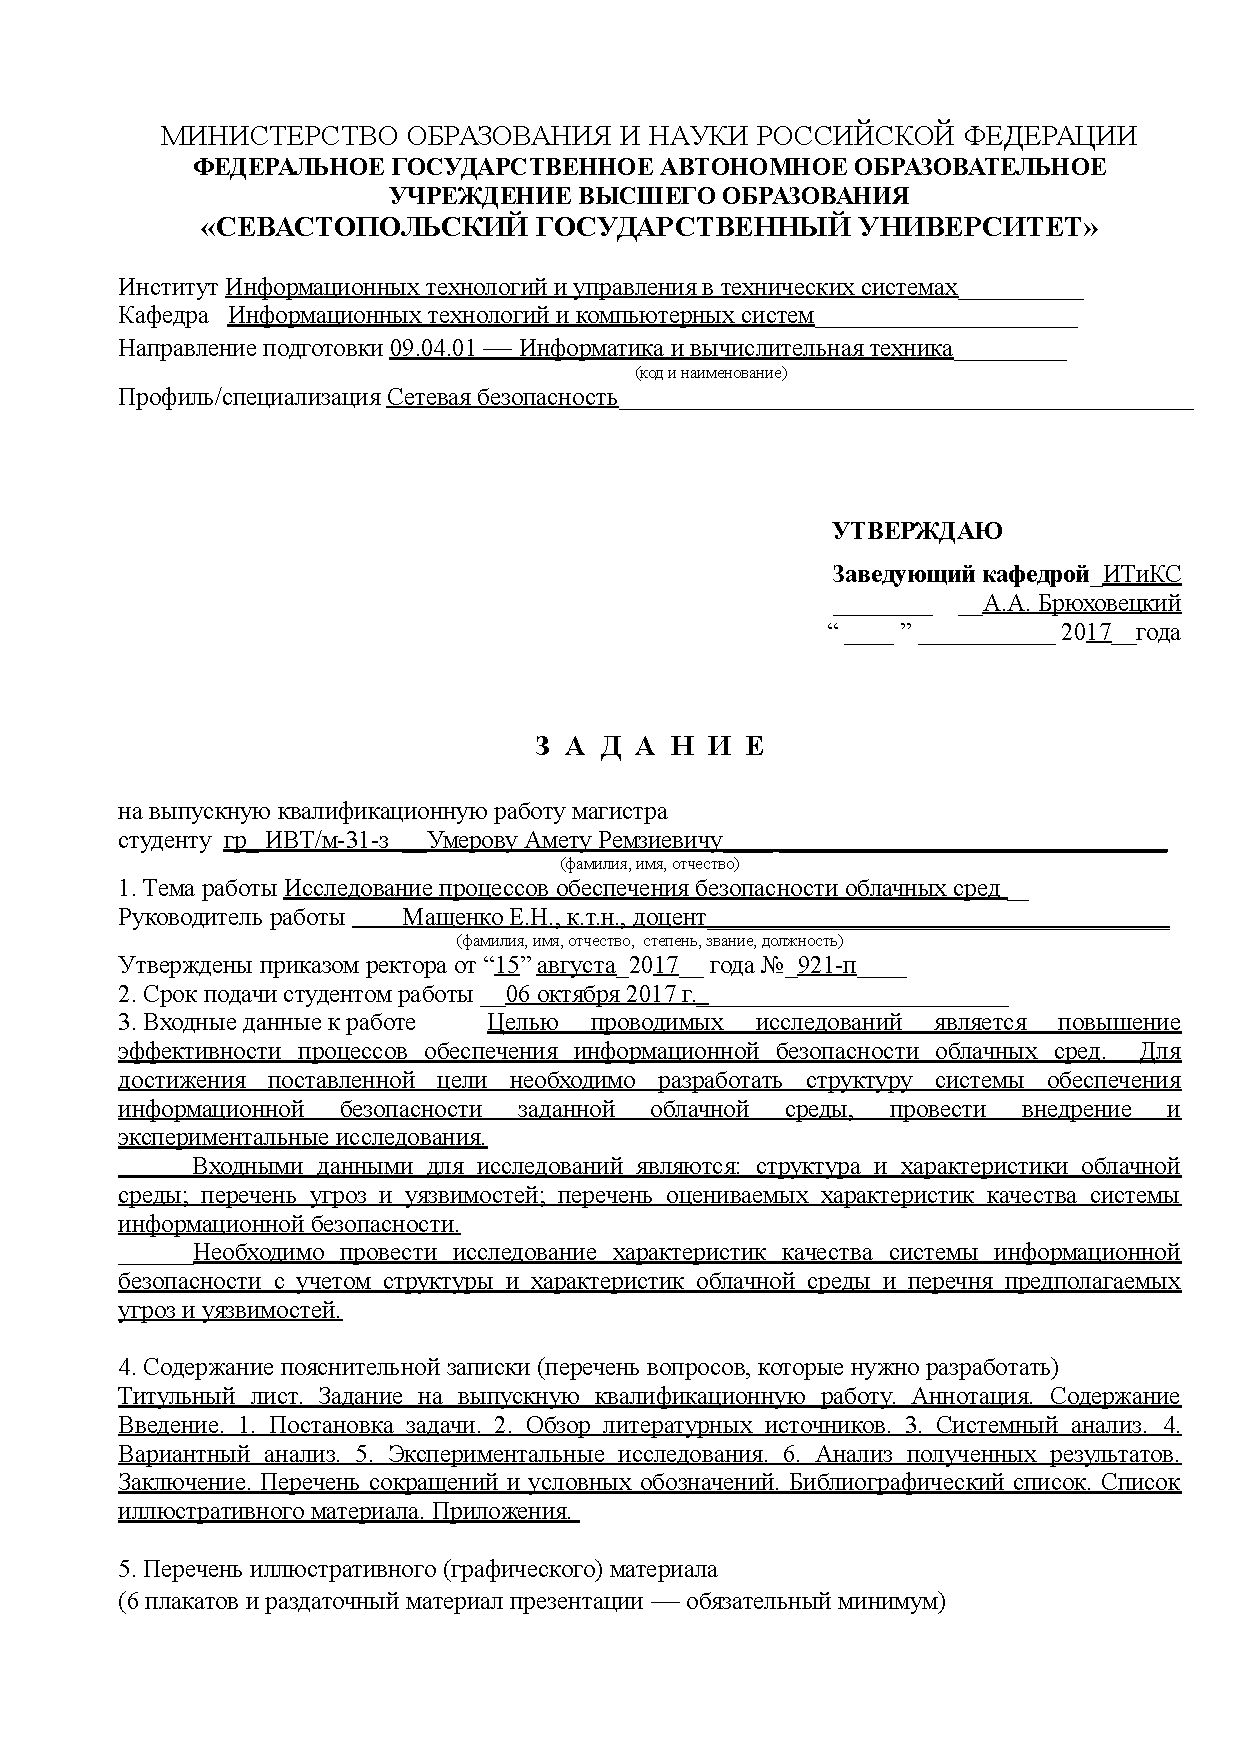
\includepdf[pages={1,2}]{task} % Задание на диплом печатается на одном листе с двух сторон
%помимо ПЗ и задания, в диплом также вкладывается отзыв руководителя и рецензия

\annotation{Аннотация}

Тема выпускной квалификационной работы магистра --- <<Исследование процессов обеспечения безопасности облачных сред>>.

Ключевые слова: безопасность, виртуализация, защита информации, облачная инфраструктура, облачные вычисления, провайдер, стандартизация, уязвимости.

В данной выпускной квалификационной работе магистра рассмотрены проблемы обеспечения безопасности облачных сред, а также представлены примеры решения этих проблем.
Для достижения поставленной цели необходимо разработать структуру системы обеспечения информационной безопасности заданной облачной среды, провести внедрение и экспериментальные исследования.

Актуальность темы.
В настоящее время наблюдается стремительное развитие облачных технологий, однако для эффективной работы облачной инфраструктуры требуется ее эффективная структура и организация.
Зачастую небольшая команда, проектирующая облачную инфраструктуру не всегда может полностью учесть все аспекты безопасности, так как нет единого документа, стандартизующего механизмы обеспечения безопасности в облачной среде.
Особенно остро вопрос безопасности встал в последнее время, в связи с обнаружением большого количества критических уязвимостей в программном обеспечении и протоколах, используемых поставщиками облачных услуг.

Целью проводимых исследований является повышение эффективности процессов обеспечения информационной безопасности облачных сред.
Для достижения поставленной цели необходимо разработать структуру системы обеспечения информационной безопасности  заданной облачной среды, провести внедрение и экспериментальные исследования.

Выпускная квалификационная работа магистра изложена на \pageref{LastPage} листах, включает 16 таблиц, 11 рисунков, 1 приложение, 28 литературных источников.

\clearpage
 % Аннотация НЕ ВКЛЮЧАЕТСЯ В СОДЕРЖАНИЕ!!!! ВОЗМОЖНО ЕЕ СВЕРСТАТЬ В ЛАТЕХЕ И СОЕДИНИТЬ КАК ПДФ НАДО

\tableofcontents % Содержание 
\clearpage

\anonsection{Введение}

Тут одна страница

\clearpage
 % Введение
\section{Постановка задачи}

Конечной задачей выпускной квалификационной работы магистра на тему <<Исследование безопасности облачных сред>> является подробный анализ стандартов безопасности облачных вычислений, варианты решения данных проблем, а также технические возможности практической эксплуатации уязвимостей на нескольких уровнях работы облачной инфраструктуры.

Исследования должны состоять из следующих частей:
\begin{itemize}
  \item обзор составных частей облачной инфраструктуры;
  \item анализ технологий используемых облачными провайдерами, необходимых для построения облачной инфраструктуры;
  \item специфика применений облачных вычислений в России;
  \item исследование проблемы безопасности облачных вычислений;
  \item решение проблем безопасности облаков;
  \item практическое применение уязвимостей в облачной среде, с использованием программ, распространяющихся под свободными лицензиями, например \hyperlink{gnu}{GNU} \hyperlink{gpl}{GPL}.
\end{itemize}

Для применения практических навыков исследования уязвимостей необходима аппаратная платформа со следующими характеристиками:
\begin{itemize}
  \item процессор Intel Core\textregistered~i3 2.3 ГГц с поддержкой аппаратной виртуализации;
  \item минимальный объем \hyperlink{ram}{ОЗУ} 8 Гб, рекомендуемый --- не менее 10 Гб;
  \item минимум 15 Гб места на жестком диске (\hyperlink{ssd}{SSD});
  \item операционная система Ubuntu 16.04, CentOS 7 или Debian 8 GNU/Linux.
\end{itemize}

Данная задача также рассматривается с точки зрения системного и вариантного анализа.

Системный анализ включает в себя \cite{sys-analyz}:
\begin{itemize}
  \item системотехническое представление системы безопасности в виде <<черного ящика>>;
  \item описание входных и выходных данных;
  \item список функций, которые выполняет система безопасности;
  \item учет случайностей;
  \item декомпозицию системы и описание связей между ее элементами.
\end{itemize}

Вариантный анализ произведен исходя выбранных критериев \cite{var-analyz}:
\begin{itemize}
  \item раз;
  \item два;
  \item три;
  \item ...;
  \item последний критерий.
\end{itemize}

\clearpage
 % Постановка задачи
\section{Обзор литературных источников по тематике исследования} \label{literature}

Исторически, ситуация сложилась так, что слово <<облако>> используется в качестве метафоры сети Интернет.
Позже, оно было использовано для изображения Интернет в компьютерных сетевых диаграммах и схемах.

Облачные вычисления можно обозначить, как выделение ресурсов в облаке.
В соответствии с Национальным институтом стандартов и технологий (\hyperlink{nist}{NIST}), формальное определение облачных вычислений заключается в следующем:
<<Облачные вычисления являются моделью обеспечения повсеместного, удобного доступа по требованию по сети, общему пулу конфигурируемых вычислительных ресурсов (например сетей, серверов, систем хранения данных (\hyperlink{storage}{СХД}), приложений и услуг), которые могут быстро и с минимальными усилиями предоставлены для управления поставщиком услуг>> \cite{nist}.

Согласно опросам института Понемона в 2016 году, среди 3476 респондентов в сфере информационной безопасности из Соединенных Штатов Америки, Великобритании, Австралии, Германии, Японии, Франции, России, Индии и Бразилии, 73\% респондентов так или иначе используют облачные вычисления в своей инфраструктуре.
Особый рост внедрения облачных услуг произошел в последние 2 года \cite{gemalto}.

Хранение данных пользователей, почты и потребительских данных в облаке выросло в 2016 году по сравнению с 2014 годом (рис. \ref{cloud-data}).

\addimg{cloud-data}{1}{Использование облачных вычислений для хранения данных}{cloud-data}

Облачные вычисления являются результатом объединения большого количества технологий и связующего ПО для обеспечения ресурсов, необходимых для решения задачи, балансировки процессов, мониторинга, автоматизации и прочего.

Основными отличиями предоставления облачных услуг от <<классических>> являются (рис. \ref{cloud-tech}):
\begin{itemize}
  \item виртуализация;
  \item оркестратор;
  \item список услуг;
  \item портал самообслуживания;
  \item система тарификации и выставления счетов (биллинг).
\end{itemize}

\addimg{cloud-tech}{0.85}{Составные части облачных вычислений}{cloud-tech}

В вычислениях, виртуализация является процессом создания виртуальной (не физической) версии чего-либо, в том числе аппаратных платформ виртуального компьютера, операционных систем, устройств хранения данных и вычислительных ресурсов.

Виртуализация может быть предоставлена на различных аппаратных и программных уровнях, таких как центральный процессор, диск, память, файловые системы и прочее.
Чаще всего виртуализация используется для создания виртуальных машин и эмуляции различного оборудования для последующей установки операционных систем (\hyperlink{os}{ОС}) на них.

Виртуальные машины создаются на основе гипервизора, который работает поверх операционной системы хост-компьютера (физического компьютера, не виртуального).
С помощью гипервизора возможна эмуляция аппаратных средств, таких как процессор, диск, сеть, память, а также установка гостевых операционных систем на них.
Возможно создание нескольких гостевых виртуальных машин с различными операционными системами на гипервизоре.
Например, можно взять машину на Linux и установить ее на <<голое>> железо (bare-metal), и после настройки гипервизора возможно создание нескольких гостевых машин на Linux и Windows.

На данный момент все современные процессоры поддерживают аппаратную виртуализацию, это необходимо для безопасного и эффективного обмена ресурсами между хост-системой и гостевыми системами.
Большинство современных процессоров и гипервизоров также поддерживают вложенную виртуализацию, что позволяет создавать виртуальные машины внутри виртуальных машин.

Оркестратор является механизмом, выполняющий набор заданных операций по шаблону.
В сервис-ориентированной архитектуре (\hyperlink{soa}{SOA}), оркестровка сервисов реализуется согласно стандарту BPEL.
Это позволяет автоматизировать процессы создания услуг пользователей в облачной среде.

Список услуг предоставляется пользователю в виде шаблонов готовых тарифов на портале самообслуживания, однако существуют и так называемые <<конфигураторы>>, которые позволяют пользователю создать шаблон индивидуально.

Портал самообслуживания является инструментом, с которым работает непосредственно пользователь.
Именно на портале обслуживания размещается список услуг, доступных пользователю.

Система тарификации и выставления счетов является необходимым механизмом для определения финансовых затрат пользователя в соответствии с затраченными ресурсами пользователя.

Поставщики облачных услуг (провайдеры) предлагают различные виды услуг, построенных поверх базового резервирования и освобождения ресурсов.
Большинство из этих услуг попадают в одну из следующих категорий (рис. \ref{aas}):
\begin{itemize}
  \item инфраструктура как услуга (IaaS);
  \item платформа как услуга (PaaS);
  \item программное обеспечение как услуга (SaaS).
\end{itemize}

\addimg{aas}{1}{Модели обслуживания облака}{aas}

Большинство поставщики облачных услуг используют различные виды веб-интерфейса, на основе которого можно построить необходимый стек технологий.
Облачные провайдеры используют модель <<pay-as-you-go>>, в которой оплата производится только за время использования ресурсов.

Ключевыми функциями облачных вычислений являются:
\begin{itemize}
  \item высокая скорость и гибкая масштабируемость;
  \item низкая стоимость;
  \item легкий доступ к ресурсам;
  \item отсутствие необходимости в обслуживании;
  \item совместное использование;
  \item надежность.
\end{itemize}

Доступ к необходимым ресурсам можно получить одним щелчком мыши, что экономит время и обеспечивает гибкость.
В зависимости от потребностей услуги, можно легко масштабировать ресурсы как горизонтально, так и вертикально.
Снижение первоначальных затрат на развертывание инфраструктуры позволяет сосредоточиться на приложениях и бизнесе, облачные провайдеры имеют возможность заранее оценить стоимость, что значительно облегчает планирование бюджета.
Пользователи могут получить доступ к инфраструктуре из любого места и устройства, до тех пор, пока существует интернет-подключение к поставщику.
Все работы по техническому обслуживанию ресурсов осуществляются поставщиком облачных услуг, пользователи не должны беспокоиться об этом.
Несколько пользователей могут использовать один и тот же пул доступных ресурсов.
Ресурсы могут быть размещены в разных дата-центрах, для обеспечения повышенной надежности.

Широкое применение облачных вычислений позволяет использовать различиные сценарии его использования.
Как правило, <<облако>> может быть развернуто согласно следующим моделям (рис. \ref{clouds}):
\begin{itemize}
  \item частное облако;
  \item публичное облако;
  \item общественное облако;
  \item гибридное облако.
\end{itemize}

\addimg{clouds}{1}{Модели развертывания облака}{clouds}

Частное облако эксплуатируется исключительно одной организацией, оно может быть размещено внутри или снаружи сети организации и управляться внутренними командами или третьей стороной.
Частное облако можно построить с использованием такого программного обеспечения, как OpenStack.

Публичное облако доступно для всех пользователей, любой может использовать его после предоставления платежных данных.
\hyperlink{aws}{AWS} (Amazon Web Services) и \hyperlink{gce}{GCE} (Google Compute Engine) являются примерами публичных облаков.

Гибридное облако является результатом объединения публичного и частных облаков.
Гибридное облако может быть использовано для хранения секретной информации о частном облаке, предлагая при этом услуги на основе этой информации из публичного облака.

Общественное облако, как правило, предназначено для сообщества или организации.

Облачные технологии относительно недавно вышли на рынок массового потребления, поэтому пока еще не существует четких общепринятых стандартов в сфере предоставления облачных услуг и обеспечении безопасности.
Поставщики облачных услуг обходят эту проблему тремя путями.

Во-первых, облачные провайдеры создают собственные корпоративные стандарты, которые чаще всего публично не оглашаются.
В таком случае потребитель может полагаться исключительно на репутацию компании, предоставляющей облачные услуги.
Среди таких компаний можно выделить Google, Amazon, Microsoft, IBM, VMWare, Oracle и прочие.
Однако такие как компании как IBM, участвуют в открытии облачных стандартов.

Во-вторых, компании адаптируют свои услуги согласно существующим и устоявшимся стандартам безопасности, проходят соответствующие сертификации с последующим получием свидетельства.
Получение подобных сертификатов актуально в плане получения государственных и общественных заказов в долгосрочной перспективе \cite{itmo}.

В-третьих, различные правительственные, коммерческие и общественные организации принимают всяческие усилия по выработке требований к созданию безопасных облачных служб обработки информации.

Рабочая группа Object Management Group (\hyperlink{omg}{OMG}) в 2009 году была инициатором создания Cloud Standarts Summit.
Целью создания встречи является развитие информационных технологий (\hyperlink{it}{ИТ}) и согласование стандартов по проблемам государственных облачных сред.
В результате были созданы следующие рабочие группы:
\begin{itemize}
  \item Cloud Security Alliance (\hyperlink{csa}{CSA});
  \item Distributed Management Task Force (\hyperlink{dmtf}{DMTF});
  \item Storage Networking Industry Association (\hyperlink{snia}{SNIA});
  \item Open Grid Forum (\hyperlink{ogf}{OGF});
  \item Open Cloud Consortium (\hyperlink{occ}{OCC});
  \item Organization for the Advancement of Structured Information Standards (\hyperlink{oasis}{OASIS});
  \item TM Forum;
  \item Internet Engineering Task Force (\hyperlink{ietf}{IETF});
  \item International Telecommunications Union (\hyperlink{itu}{ITU});
  \item European Telecommunications Standards Institute (\hyperlink{etsi}{ETSI});
  \item National Institute of Standards and Technology (NIST);
  \item Object Management Group (OMG).
\end{itemize}

Наиболее известны достижения NIST, CSA, OASIS, а так же организации Open Data Center Alliance.

Cloud Security Alliance является некоммерческой организацией, созданной с целью продвижения идеи обеспечения безопасности облачных вычислений, а также для повышения уровня осведомленности по данной тематике как облачных поставщиков услуг, так и потребителей.
Ряд основных задач, выделаемых организацией CSA:
\begin{itemize}
  \item поддержка взаимоотношений потребителей и поставщиков услуг в требованиях безопасности и контроля качества;
  \item независимые исследования в части защиты;
  \item разработка и внедрение программ повышения осведомленности и обеспечению безопасности;
  \item разработка руководств и методических рекомендаций по обеспечению безопасности.
\end{itemize}

Руководство по безопасности критических областей в области облачных вычислений (Security Guidance for Critical Areas of Focus in Cloud Computing) покрывает основные аспекты и дает рекомендации потребителям облачных сред в тринадцати стратегически важных областях:
\begin{itemize}
  \item архитектурные решения сред облачных вычислений;
  \item государственное и корпоративное управление рисками;
  \item легальное и электронное открытие;
  \item соответствие техническим условиям и отчетность;
  \item управление жизненным циклом информации;
  \item портативность и совместимость;
  \item традиционная безопасность, непрерывность деятельности и восстановление в аварийных ситуациях;
  \item работа центра обработки данных;
  \item реакция на риски, уведомление и коррекционное обучение;
  \item прикладная безопасность;
  \item криптография и управление ключами;
  \item идентификация и управление доступом;
  \item виртуализация.
\end{itemize}

OASIS стимулирует развитие, сведение и принятие открытых стандартов для глобального информационного общества. Являясь источником многих современных основополагающих стандартов, организация видит облачные вычисления как естественное расширение сервисноориентированной архитектуры и моделей управления сетью \cite{psta}.
Технические агенты OASIS –– это набор участников, многие из которых активно участвуют в построении моделей облаков, профилей и расширений на существующие стандарты.
Примерами стандартов, разработанных в области политик безопасности, доступа и идентификации, являются OASIS SAML, XACML, SPML, WS-SecurityPolicy, WS-Trust, WS-Federation, KMIP и ORMS.

Организация Open Data Center Alliance объявила о публикации двух моделей использования (usage models), призванных снять наиболее значимые препятствия на пути внедрения облачных вычислений.
Первая модель использования называется <<The Provider Security Assurance>> (обеспечение безопасности на стороне поставщика облачных услуг).
В ней описаны требования к гранулированному описанию элементов обеспечения безопасности, которые должны предоставить поставщики услуг.

Вторая модель использования <<The Security Monitoring>> (мониторинг соответствия требованиям безопасности) описывает требования к элементам, которые обеспечивают возможность мониторинга безопасности облачных услуг в реальном времени.
В совокупности две модели использования формируют набор требований, который может стать основой для создания стандартной модели обеспечения безопасности облачных услуг и осуществления мониторинга этих услуг в реальном времени.

Национальный Институт стандартов и технологий вместе с Американским национальным институтом стандартов (ANSI) участвует в разработке стандартов и спецификаций к программным решениям, используемым как в государственном секторе США, так и имеющим коммерческое применение.
Сотрудники NIST разрабатывают руководства, направленные на описание архитектуры облака, безопасность и стратегии использования, в числе которых руководство по системам обнаружения и предотвращения вторжений, руководство по безопасности и защите персональных данных при использовании публичных систем облачных вычислений.

В руководстве по системам обнаружения и предотвращения вторжений (NIST Guide to Intrusion Detection and Prevention Systems) даются характеристики технологий \hyperlink{idps}{IDPS} (Intrusion Detection and Prevention Systems) и рекомендации по их проектированию, внедрению, настройке, обслуживанию, мониторингу и поддержке.
Виды технологий IDPS различаются в основном по типам событий, за которыми проводится наблюдение, и по способам их применения.
Рассмотрены следующие четыре типа IDPS-технологий: сетевые, беспроводные, анализирующие поведение сети и централизованные.

В руководстве по безопасности и защите персональных данных при использовании публичных систем облачных вычислений в том числе дается обзор проблем безопасности и конфиденциальности, имеющих отношение к среде облачных вычислений: обнаружение атак на гипервизор, цели атак, отдельно рассматриваются распределенные сетевые атаки.

Инфраструктура как услуга является одной из форм облачных вычислений, которая обеспечивает доступ по требованию к физическим и виртуальным вычислительным ресурсам, сети, межсетевым экранам, балансировщикам нагрузки и так далее.
Для обеспечения виртуальными вычислительными ресурсами, IaaS использует различные формы гипервизоров, таких как Xen, KVM, VMWare ESX/ESXi, Hyper-V и прочие.

Amazon Web Services является одним из лидеров в области предоставления услуг различных облачных сервисов.
С помощью Amazon Elastic Compute Cloud (\hyperlink{ec2}{EC2}), Amazon предоставляет пользователям IaaS-инфраструктуру (рис. \ref{ec2}).
Пользователь может управлять вычислительными ресурсами (инстансами) через веб-интерфейс Amazon EC2.
Существует возможность горизонтального и вертикального масштабирования ресурсов, в зависимости от требований.
AWS также предоставляет возможность управления инстансами посредством интерфейса командной строки и с помощью Application Programming Interface (\hyperlink{api}{API}).

\addimg{ec2}{1}{Сценарий построения инфраструктуры компании на основе EC2}{ec2}

В качестве гипервизора, Amazon EC2 использует Xen \cite{xen}.
Серввис предлагает инстансы различных конфигураций, которые можно выбрать в зависимости от требований.
Некоторые примеры различных конфигураций инстансов:
\begin{itemize}
  \item t2.nano: 512 Мб ОЗУ, 1 \hyperlink{vcpu}{vCPU} (виртуальных процессорных ядер), 32 или 64-битные платформы;
  \item c4.large: 4 Гб ОЗУ, 2 vCPU, 64-битная платформа;
  \item d2.8xlarge: 256 Гб ОЗУ, 36 vCPU, 64-битная платформа, 10G Ethernet.
\end{itemize}

Amazon EC2 предоставляет некоторые предварительно настроенные образы операционных систем, называемые Amazon Machine Images (\hyperlink{ami}{AMI}).
Эти образы могут быть использованы для быстрого запуска инстансов.
Пользователь также может создавать собственные образы ОС.
Amazon поддерживает настройки безопасности и доступа к сети для пользовательских инстансов.
С помощью Amazon Elastic Block Store (\hyperlink{ebs}{EBS}) пользователь может монтировать хранилища данных к инстансам.

Amazon EC2 имеет много других возможностей, что позволяет:
\begin{itemize}
  \item создавать <<гибкие>> IP-адреса для автоматического переназначения статического IP-адреса;
  \item предоставлять виртуальные частные облака;
  \item использовать услуги для мониторинга ресурсов и приложений;
  \item использовать автомасштабирование для динамического изменения доступных ресурсов.
\end{itemize}

Облачная платформа Azure, поддерживаемая компанией Microsoft, предлагает большой спектр облачных услуг, таких как: вычислительные мощности, платформы для мобильной и веб-разработки, хранилища данных, интернет вещей (\hyperlink{iot}{IoT}) и другие.

DigitalOcean позиционирует себя как простой облачный хостинг.
Все виртуальные машины (дроплеты) работают под управлением гипервизора KVM и используют SSD-накопители.
DigitalOcean предоставляет и другие функции, такие как IP-адреса расположенные в пределах одного дата-центра, частные сети, командные учетные записи и прочее.
Простота веб-интерфейса, высокое качество работы виртуальных машин и доступность для обычного пользователя способствовали быстрому росту компании.

На российском рынке облачного хостинга все еще наблюдается большой рост.
В связи с тем, что нет явно выраженного монополиста, таких как Amazon, Rackspace, Terramark, российский рынок очень разнообразный.
Конкуренция на рынке способствует значительному повышению качества предоставляемых услуг, а также гибкие тарифные планы и широкий перечень дополнительных услуг.

Также важную роль играет принятие Федерального закона от 21 июля 2014 г. № 242-ФЗ <<О внесении изменений в отдельные законодательные акты Российской Федерации в части уточнения порядка обработки персональных данных в информационно-телекоммуникационных сетях>> \cite{minsvyaz}.
Крупные компании обязаны хранить персональные данные пользователй на территории России, что способствует консолидации российского рынка облачных услуг.

Крупнейшие поставщики услуг ЦОД 2016 г. \cite{cnews} представлены в табл. \ref{dc-table}.
\begin{table}[H]
  \caption{Крупнейшие поставщики услуг ЦОД в 2016 году}\label{dc-table}
  \begin{tabular}{|p{0.6cm}|p{2.6cm}|p{3cm}|p{3.5cm}|p{3.5cm}|}
  \hline \# & Название компании & Количество доступных стойко-мест & Количество размещенных стойко-мест & Загруженность мощностей (\%) \\
  \hline 1 & Ростелеком & 3 900 & 3 432 & 88 \\
  \hline 2 & DataLine & 3 703 & 2 988 & 81 \\
  \hline 3 & DataPro & 3 000 & н/д & н/д \\
  \hline 4 & Linxtelecom & 2 040 & н/д & н/д \\
  \hline 5 & Selectel & 1 500 & 1 200 & 80 \\
  \hline 6 & Stack Group & 1 400 & 854 & 61 \\
  \hline 7 & Ай-Теко & 1 200 & 960 & 80 \\
  \hline 8 & DataSpace & 1 152 & 820 & 71 \\
  \hline 9 & SDN & 1 074 & 815 & 76 \\
  \hline 10 & Крок & 1 000 & 980 & 98 \\
  \hline
  \end{tabular}
\end{table}

Данные DataLine включают показатели 7 ЦОД, расположенных на площадказ OST и NORD.
Данные по количеству введенных в эксплуатацию и реально размещенных стоек в ЦОД DataPro и Linxtelecom отсутствуют.

По итогам 2015 г. CNews Analytics впервые составил рейтинг крупнейших поставщиков IaaS.
В исследовании приняли участие 14 компаний, совокупная выручка которых составила 3,8 млрд. рублей.
По сравнению с 2014 г. участники заработали на 63\% больше.
Все участники рейтинга продемонстрировали положительную динамику за исключением компании Inoventica (-3\%).
Высокие темпы роста свидетельствуют о том, что рынок IaaS находится в начале своего становления.
Многие участники рейтинга вышли на этот рынок только в 2014-2015 г., чем объяснятся наличие большого числа компаний с ростом более в чем 3 раза: StackGroup (+733\%), 1cloud.ru (+911\%), CaravanAero (+1220\%).

Сравнение крупнейших поставщиков IaaS в 2016 г. \cite{cnews} представлено в табл. \ref{iaas-table}.
\begin{table}[H]
  \caption{Крупнейшие поставщики IaaS в 2016 году}\label{iaas-table}
  \begin{tabular}{|p{0.5cm}|p{2.5cm}|p{3.5cm}|p{3.5cm}|p{4.5cm}|}
  \hline \# & Название компании & Выручка IaaS в 2015 г. (тыс.р.) & Выручка IaaS в 2014 г. (тыс.р.) & ЦОД \\
  \hline 1 & ИТ-Град & 857 245 & 358 680 & Datalahti, DataSpace, SDN, AHOST \\
  \hline 2 & Крок & 667 609 & 440 315 & Волочаевская-1/2, Компрессор \\
  \hline 3 & Ай-Теко & 618 500 & 565 800 & ТрастИнфо \\
  \hline 4 & DataLine & 500 960 & 358 400 & NORD1/2/3/4, OST1/2/3 \\
  \hline 5 & SoftLine & 367 000 & 152 000 & н/д \\
  \hline 6 & Cloud4Y & 304 600 & 267 400 & Цветочная, М8/9/10, Nord, Equinix FR5, EvoSwitch \\
  \hline 7 & Stack Group & 182 900 & 21 948 & M1 \\
  \hline 8 & ActiveCloud & 103 702 & 56 910 & DataLine \\
  \hline 9 & Inoventica & 79 000 & 81 000 & н/д \\
  \hline 10 & 1cloud.ru & 78 307 & 7 743 & SDN, DataSpace \\
  \hline
  \end{tabular}
\end{table}

Почти все участники рейтинга SaaS продемонстрировали положительную динамику выручки, при этом у 10 компаний оборот вырос более чем на 50\%, а четыре поставщика облачных услуг зафиксировали рост выручки более чем на 100\%: Naumen (+358\%), amoCRM (+159\%), ИТ-Град (+134\%) и Artsofte (+125\%).

Сравнение крупнейших поставщиков SaaS в 2016 г. \cite{cnews} представлено в табл. \ref{saas-table}.
\begin{table}[H]
  \caption{Крупнейшие поставщики SaaS в 2016 году}\label{saas-table}
  \begin{tabular}{|p{0.5cm}|p{3.5cm}|p{3.5cm}|p{3.5cm}|p{3.5cm}|}
  \hline \# & Название компании & Выручка SaaS в 2015 г. (тыс.р.) & Выручка SaaS в 2014 г. (тыс.р.) & Рост выручки 2015/2014 (\%) \\
  \hline 1 & СКБ Контур & 6 970 000 & 5 500 000 & 27 \\
  \hline 2 & Манго Телеком & 1 808 000 & 1 350 000 & 34 \\
  \hline 3 & B2B-Center & 1 163 300 & 1 155 842 & 1 \\
  \hline 4 & Барс Груп & 1 074 000 & 910 000 & 18 \\
  \hline 5 & SoftLine & 1 034 000 & 636 000 & 63 \\
  \hline 6 & Корпус Консалтинг СНГ & 783 511 & 602 825 & 32 \\
  \hline 7 & Terrasoft & 657 654 & 476 561 & 38 \\
  \hline 8 & Телфин & 398 500 & 317 900 & 25 \\
  \hline 9 & МойСклад & 395 000 & 265 000 & 49 \\
  \hline 10 & ИТ-Град & 265 400 & 113 420 & 134 \\
  \hline
  \end{tabular}
\end{table}

В настоящее время одними из основных трендов в сфере ИТ, в частности в облачных вычислениях являются <<зеленые>> центры обработки данных и программно-конфигурируемые сети или Software-defined Networking (\hyperlink{sdn}{SDN}).

Все центры обработки данных сталкиваются с проблемой вывода тепловой энергии.
Тепловая энергия являет побочным действием от эксплуатации плотно укомплектованных серверных стоек.
Для охлаждения ЦОД необходимо большое количество холодильных установок, которые потребляют количество энергии сравнимое с некоторыми городами \cite{cnewsdc}.
Крупные компании хотят строить центры обработки данных в северных странах, таких как Исландия и Финляндия, однако удаленность от крупных магистральных сетевых точек и недостаток квалифицированных кадров для обслуживания ЦОД замедляют данный тренд.
Тепло, выделяемое дата-центром можно использовать для обогрева близлежащих жилых комплексов.
Возможность заново использовать излишнее тепло от серверов предусматривается на этапе разработки нового ЦОД, помогая повысить энергетическую эффективность оборудования.

Одной из главных расходных статей в проектировании центров обработки данных таких крупных компаний как Google, Amazon, eBay, Microsoft, является электроэнергия.
В 2008 году компания McKinsey \& Company провела аналитический обзор выбросов углекислого газа от выработки электроэнергии для нужд ЦОД \cite{greendc}.
Согласно исследованиям, суммарные показатели выброса углекислого газа ЦОД сравнимы с выбросам такой страны как Аргентина.

За счет использования энергии солнца и ветра уже работает большое количество коммерческих ЦОД.
Первый в мире <<зеленый>> дата-центр, который работает исключительно на энергии ветра построен в США, в штате Иллинойс.

Компания Microsoft использует контейнеры в качестве здания для ЦОД.
Таким образом такие контейнеры легко переносить к источникам возобновляемой энергии, за счет этого выбросы углекислого газа в атмосферу значительно сокращаются.

Также Microsoft в рамках Project Natick создала прототип ЦОД под названием Leona Philpot.
Прототип был погружен в США, недалеко от Тихого океана и успешно проработал на протяжении четырех месяцев.
Большое количество теплообменников, которыми был оснащен Leona Philpot, передавали лишнее тепло от серверов в воду.
При этом по оценкам экологов, это не влияет на глобальное повышение на температуру воды в мировом океане.

Основными трендами развития корпоративных сетей и сетей центров обработки данных являются:
\begin{itemize}
  \item рост объемов трафика, изменение структуры трафика;
  \item рост числа пользователей мобильных приложений и социальных сетей;
  \item высокопроизводительные кластеры для обработки большого количества данных;
  \item виртуализация для предоставления облачных услуг.
\end{itemize}

Программно-конфигурируемая сеть --- форма виртуализации вычислительных ресурсов (сети), в которой уровень управления отделен от уровня передачи данных (рис. \ref{vnet}).
Основным преимуществом такой сети является то, что большое количество сетей возможно программно объединить в одну и централизованно управлять ею.

\addimg{vnet}{1}{Схема программно-конфигурируемой сети}{vnet}

Если рассмотреть современный маршрутизатор или коммутатор, то логически его можно разделить на три компонента:
\begin{itemize}
  \item уровень управления;
  \item уровень управления трафиком;
  \item передача трафика.
\end{itemize}

На уровне управления присутствует командный интерфейс, программная оболочка, протоколы управления или встроенный веб-сервер.
Основная задача уровня управления --- обеспечить управляение устройством.
На уровень управления трафиком приходятся алгоритмы.
Функциональная задача данного уровня --- автоматическая реакция на изменение трафика.
Функционал передачи трафика обеспечивает физическую передачу данных на низших уровнях.

Для построения программно-конфигурируемых сетей используется стандартный протокол OpenFlow.
Большое количество коммутаторов уже поддерживает этот протокол.
Крупные вендоры сетевого оборудования, такие как Hewlet-Packard, считают что развитие SDN и в частности протокола OpenFlow позволит возобновить процесс внедрения инноваций в уже давно устоявшейся области сетевых технологий.

\clearpage
 % Обзор литературных источников по тематике исследования
\section{Системный анализ}

На данный момент при анализе и синтезе сложных программных и аппаратных систем все чаще используется системный подход.
Важным моментом для системного подхода является определение структуры системы --- совокупности связей между элементами системы, отражающих их взаимодействие.

Принципы системного анализа --- это положения общего характера, являющиеся обобщением опыта работы человека со сложными системами.
Пренебрежение принципами при проектировании любой нетривиальной технической системы, непременно приводит к потерям того или иного характера, от увеличения затрат в процессе проектирования до снижения качества и эффективности конечного продукта.

Системный анализ выполнен в соответствии с \cite{sys-analyz}.

\subsection{Принцип конечной цели} \label{goal}

Принцип конечной цели --- основополагающий принцип системного анализа.
Конечная цель имеет абсолютный приоритет, в системе все должно быть подчинено достижению конечной цели.
Принцип имеет несколько правил:
\begin{itemize}
  \item для проведения системного анализа необходимо в первую очередь, сформулировать цель функционирования системы, так как расплывчатые, не полностью определенные цели влекут за собой неверные выводы;
  \item анализ системы следует вести на базе первоочередного уяснения основной цели исследуемой системы, что позволит определить ее существенные свойства, показатели качества и критерии оценки;
  \item при синтезе систем любая попытка изменения или совершенствования должна быть в первую очередь рассмотрена с позиции его полезности в достижении конечной цели;
  \item цель функционирования искусственной системы задается, как правило, системой, в которой исследуемая система является составной частью.
\end{itemize}

В соответствии с данным принципом должна быть четко сформулирована конечная цель --- назначение проектируемой системы и сформирован список функций, которые должна выполнять система.

Цель проектирования --- разработка системы безопасности облачной среды.
Список функций проектируемой системы:
\begin{itemize}
  \item Ф1 --- авторизация и аутентификация пользователей;
  \item Ф2 --- сетевая защита;
  \item Ф3 --- идентификация и обработка инцидентов связанных с безопасностью;
  \item Ф4 --- предоставление доступа к услугам;
  \item Ф5 --- мониторинг.
\end{itemize}

\subsection{Принцип единства}

Принцип единства --- это совместное рассмотрение системы как целого и как совокупности частей.
Принцип ориентирован на декомпозицию с сохранением целостных представлений о системе.
Система должна рассматриваться и как целое, и как совокупность элементов.
Расчленение системы необходимо производить, сохраняя целостное представление о системе.
Принцип подразумевает выделение подсистем, композиция которых в совокупности со связями позволяет выполнять все функции проектируемой системы, определяет ее структуру и может быть рассмотрена как единая, целостная система.

На основании функций проектируемой системы, представленных выше, в ней можно выделить следующие подсистемы:
\begin{enumerate}
  \item подсистема аутентификации;
  \item подсистема авторизации;
  \item подсистема сетевой защиты;
  \item подсистема проверки целостности данных.
\end{enumerate}

На рис. \ref{subsys} представлена схема взаимодействия между подсистемами.
\addimg{subsys}{0.8}{Взаимодействие между подсистемами и их связь с окружающей средой}{subsys}

Обозначения, приведенные на рис. \ref{subsys} требуют пояснения:
\begin{itemize}[label={}]
  \item a --- информация, предоставляемая пользователем передается на сервер;
  \item b --- выходная информация (результат выполнения);
  \item c --- проверка корректности переданных данных;
  \item d --- в случае некорректных данных авторизации, возвращается управление к подсистеме аутентификации;
  \item e --- предоставление доступов к инфраструктуре;
  \item f --- возврат информации о правах доступа пользователя;
  \item g --- обеспечение целостности данных инфраструктуры;
  \item h --- обеспечение целостности данных пользователя.
\end{itemize}

\subsection{Принцип связности и модульности}

Любая часть системы должна рассматриваться со всеми своими связями с окружающими ее объектами, как внешними по отношению ко всей системе, так и внутренними --- другими элементами системы.
Если некоторая подсистема имеет связи только с внешней средой, то есть смысл реализовать ее в виде отдельной системы.
Подсистема, не связанная ни с внешней средой, ни с другой подсистемой, является избыточной и должна быть удалена из системы.

В соответствии с принципом модульности, выделение модулей системы, если таковые имеются, продуктивно и оправдано.
Под модулями здесь понимаются относительно автономные и достаточно простые блоки, выполняющие ограниченный набор функций.
Модуль в отличие от подсистем, которые имеют нерегулярную структуру и, как правило, несут определенную функцию, частично отражающую функцию системы, имеет регулярную структуру и характерные для него внутренние и внешние связи.
Принцип указывает на возможность вместо части системы исследовать совокупность ее входных и выходных воздействий.
Выделению модулей соответствует декопмозиция сложной задачи на множество более простых подзадач.

Принцип модульности для разрабатываемой системы поясняется с помощью рис. \ref{modules}, описывающего разбиение на модули системы аутентификации.

\addimg{modules}{0.65}{Принцип модульности на примере подсистемы аутентификации}{modules}

Излишняя детализация не требуется, поэтому остальные системы на модули принято решение не разбивать.

\subsection{Принцип функциональности}

Принцип определяет первичность функции по отношению к структуре, так же, как цель первична для функции.
Другими словами, цель определяет функции системы, а функции определяют ее структуру --- совокупность элементов с их связями.
Структура же, в свою очередь, определяет параметры системы.
В случае придания системе новых функций полезно пересматривать ее структуру, а не пытаться втиснуть новую функцию в старую схему.
Поскольку выполняемые функции составляют процессы, то целесообразно рассматривать отдельно процессы, функции, структуры.

Функции подсистем приведены в пункте \ref{goal}.

Матрица инциденций функций системы и функций назначения подсистем приведена в табл. \ref{inc-matrix}.
\begin{table}[H]
  \caption{Матрица инциденций}\label{inc-matrix}
  \begin{tabular}{|c|c|c|c|c|c|}
  \hline \multirow{2}{*}{Функции} & \multicolumn{4}{|c|}{Подсистемы} & \multirow{2}{*}{Инфраструктура} \\
  \cline{2-5} & 1 & 2 & 3 & 4 & \\
  \hline Ф1 & + & + & & & + \\
  \hline Ф2 & & & + & & + \\
  \hline Ф3 & & + & & & + \\
  \hline Ф4 & + & + & + & + & + \\
  \hline Ф5 & + & + & + & + & + \\
  \hline
  \end{tabular}
\end{table}

В матрице инциденций знаком <<+>> обозначены функции, которые реализуются для каждой из подсистем.

Детализация функций подсистемы на примере подсистемы аутентификации:
\begin{enumerate}
  \item обеспечение возможности ввода данных (веб-интерфейс или API);
  \item обеспечение шифрованного канала для передачи данных;
  \item сверка полученных данных с внутренней базой;
  \item возможность восстановления доступов с помощью двухфакторной аутентификации.
\end{enumerate}

Входными данными для подсистемы является информация о пользователе, а выходными --- подтвержденный вход пользователя.

\subsection{Принцип иерархии}

Разработка иерархий классов является нетривиальной задачей.
Грамотно спроектированные иерархии классов позволяют создавать высокоэффективные системы, плохо спроектированная иерархия приводит к созданию сложных и запутанных систем.

Выполнение принципа иерархичности для разрабатываемой системы на примере подсистемы проверки целостности данных проиллюстрировано на рис. \ref{hierarchy}.
\addimg{hierarchy}{1}{Принцип иерархии на примере подсистемы обеспечения целостности данных}{hierarchy}

\subsection{Принцип сочетания централизации и децентрализации}

Степень централизации должна быть минимальной, обеспечивающей выполнение поставленной цели.
Соотношение централизации и децентрализации определяется уровнями, на которых вырабатываются и принимаются управленческие решения.

Недостатком децентрализованного управления является увеличение времени адаптации системы, которое существенно влияет на функционирование системы в быстро меняющихся средах.
То, что в централизованных системах можно сделать за короткий промежуток времени, в децентрализованной системе будет осуществляться весьма медленно.
Недостатком централизованного управления является сложность управления из-за огромного потока информации, подлежащей переработке в старшей системе управления.
В медленно меняющейся обстановке децентрализованная часть системы успешно справляется с адаптацией поведения системы к среде и с достижением глобальной цели системы за счет оперативного управления, а при резких изменениях среды осуществляется централизованное управление по переводу системы в новое состояние.

Например, можно выполнить декомпозицию подсистемы сетевой защиты таким образом:
\begin{enumerate}
  \item подсистема работы виртуальной частной сети (\hyperlink{vpn}{VPN});
  \item подсистема защиты от атак на отказ;
  \item подсистема работы межсетевого экрана.
\end{enumerate}

Такое разбиение позволит реализовать полученные подмножества в виде отдельных модулей.

\subsection{Принцип развития}

Учет изменяемости системы, ее способности к развитию, адаптации, расширению, замене частей, накапливанию информации.
В основу синтезируемой системы требуется закладывать возможность развития, наращивания усовершенствования.
Обычно расширение функций предусматривается за счет обеспечения возможности включения новых модулей, совместимых с уже имеющимися.
С другой стороны, при анализе принцип развития ориентирует на необходимость учета предыстории развития системы и тенденций, имеющихся в настоящее время, для вскрытия закономерностей ее функционирования.

Одним из способов учета этого принципа разработчиками является рассмотрение системы относительно ее жизненного цикла.
Условными фазами жизненного цикла являются: проектирование, изготовление, ввод в эксплуатацию, эксплуатация, наращивание возможностей (модернизация), вывод из эксплуатации (замена), уничтожение.

Отдельные авторы этот принцип называют принципом изменения (историчности) или открытости.
Для того чтобы система функционировала, она должна изменяться, взаимодействовать со средой.

Проектируемая система может быть развита:
\begin{itemize}
  \item переходом на более гибкие файловые системы;
  \item внедрением дополнительных технологий виртуализации;
  \item увеличением штата системных инженеров;
  \item введением расширенного мониторинга;
  \item многоуровневой защитой от атак на отказ;
  \item расширением памяти на системах хранения данных;
  \item многоуровневой репликацией и резервным копированием.
\end{itemize}

\subsection{Принцип учета случайностей}

Можно иметь дело с системой, в которой структура, функционирование или внешние воздействия не полностью определены.

Сложные системы не всегда подчиняются вероятностным законам.
В таких системах можно оценивать <<наихудшие>> ситуации и проводить рассмотрение для них.
Этот способ обычно называют методом гарантируемого результата, он применим, когда неопределенность не описывается аппаратом теории вероятностей.

События и действия, некорректные с точки зрения правил функционирования системы:
\begin{itemize}
  \item попытка входа без использования двухфакторной аутентификации;
  \item сбой в работе аппаратуры, в частности устройств хранения данных;
  \item сбой сети в в пределах дата-центра или на магистрали;
  \item отсутствие своевременной работы системных инженеров;
  \item ошибки и уязвимости в используемых программных платформах.
\end{itemize}

Кроме того, необходимо вести контроль успешности и целостности проведения операций с компонентами системы, данными пользователей и корректно обрабатывать исключения, возникновение которых возможно в процессе работы системы.

Перечисленные выше принципы обладают высокой степенью общности.
Такая интерпретация может привести к обоснованному выводу о незначимости какого-либо принципа.
Однако, знание и учет принципов позволяет лучше увидеть существенные стороны решаемой проблемы, учесть весь комплекс взаимосвязей, обеспечить системную интеграцию.

\clearpage
 % Системный анализ
\section{Вариантный анализ}

Выберем среду имитационного моделирования при помощи метода анализа иерархии (МАИ).
Метод состоит в разложении проблемы на все более простые составные части и дальнейшей обработке последовательных суждений лица принимающего решение по парным сравнениям.
В результате может быть выражена интенсивность или относительная степень взаимодействия элементов в иерархии.
В результате получаются численные выражения этих суждений.
МАИ включает в себя процедуры синтеза множественных суждений, получение приоритетных критериев и нахождение альтернативных решений.
Полученные знания являются оценками в шкале отношений и соответствуют жёстким оценкам [4].

В качестве альтернатив используются различные среды имитационного моделирования, на которых может быть реализована система защиты.
В зависимости от выбранной среды будет выбран тот или другой интерфейс взаимодействия с пользователем, так как каждая система имеет в своем составе такой интерфейс.
Критерием эффективности является доступность, простота использования, интерфейс проектируемой системы, анимация, возможность изменения параметров моделируемой системы.

Альтернативы, которые участвуют в вариантном анализе:
\begin{itemize}
  \item Arena (альтернатива А);
  \item GPSS (Альтернатива Б);
  \item AnyLogic (Альтернатива В).
\end{itemize}

Критерии, по которым выбирается тот, или иной алгоритм:
\begin{itemize}
  \item доступность (А1);
  \item простота (А2);
  \item интерфейс модели (А3);
  \item анимация (А4);
  \item внесение изменений в модель (А5).
\end{itemize}

\subsection{Построение матриц парных сравнений второго уровня}

На основе вышеперечисленных критериев построим матрицу парных сравнений второго уровня, где строки и столбцы составляют выбранные критерии.
Сравнение критериев проведём по шкале относительной важности согласно с табл. \ref{crit}.
\begin{table}[H]
  \caption{Оценка критериев}\label{crit}
  \begin{tabular}{|p{4cm}|p{12cm}|}
  \hline Интенсивность относительной важности & \multicolumn{1}{|c|}{Определение} \\
  \hline 1 & если элементы $A_i$ и $A_k$ одинаково важны \\
  \hline 3 & если элементы $A_i$ и $A_k$ одинаково важны \\
  \hline 5 & если элемент $A_i$ значительно важнее элемента $A_k$ \\
  \hline 7 & если элемент $A_i$ явно важнее элемента $A_k$ \\
  \hline 9 & если элемент $A_i$ по своей значимости абсолютно превосходит элемент $A_k$ \\
  \hline 2,4,6,8 & используются для облегчения компромиссов между оценками, слегка отличающимися от основных чисел \\
  \hline
  \end{tabular}
\end{table}

В результате выполнения попарных сравнений, построили матрицу, представленную в табл. \ref{matrix}.
\begin{table}[H]
  \caption{Матрица попарных сравнений второго уровня}\label{matrix}
  \begin{tabular}{|p{0.6cm}|p{8cm}|l|l|l|l|l|}
  \hline \multicolumn{2}{|c|}{Критерии} & A1 & A2 & A3 & A4 & A5 \\
  \hline A1 & Доступность & 1 & 1/5 & 1/7 & 1/5 & 1/7 \\
  \hline A2 & Простота & 5 & 1 & 1/5 & 3 & 1 \\
  \hline A3 & Интерфейс модели & 7 & 5 & 1 & 5 & 5 \\
  \hline A4 & Анимация & 5 & 1/3 & 1/5 & 1 & 1/7 \\
  \hline A5 & Внесение изменений в модель & 7 & 1 & 1/5 & 7 & 1 \\
  \hline
  \end{tabular}
\end{table}

\subsection{Вычисление вектора приоритетов для матрицы парных сравнений второго уровня}

Из группы матриц попарных сравнений формируется набор локальных приоритетов, которые выражают относительное влияние множества элементов на элемент примыкающего сверху уровня.
Сначала вычислим геометрическое среднее в каждой строке матрицы A по формуле:
\begin{equation}
b_i = \sqrt[n]{\prod_{k=1}^{n}a_{ik}}
\end{equation}

Проведем вычисления компонент вектора локальных приоритетов:

$b_1 = \sqrt[5]{1 \cdot 0,2 \cdot 0,1429 \cdot 0,2 \cdot 0,1429} = \sqrt[5]{0,0007} = 0,2339$

$b_2 = \sqrt[5]{5 \cdot 1 \cdot 0,2 \cdot 3 \cdot 1} = \sqrt[5]{3} = 1,2457$

$b_3 = \sqrt[5]{7 \cdot 5 \cdot 1 \cdot 5 \cdot 5} = \sqrt[5]{875} = 3,8762$

$b_4 = \sqrt[5]{5 \cdot 0,3333 \cdot 0,2 \cdot 1 \cdot 0,1429} = \sqrt[5]{0,0476} = 0,5439$

$b_5 = \sqrt[5]{7 \cdot 1 \cdot 0,2 \cdot 7 \cdot 1} = \sqrt[5]{9,8} = 1,5785$

Просуммируем полученные значения:

$B = 0,2339 + 1,2457 + 3,8762 + 0,5439 + 1,5785 = 7,4782$

Определим значения компонент вектора локальных приоритетов по формуле:
\begin{equation}
x_i = \frac{b_i}{B}, i = \overline{1,n}
\end{equation}

Выполним расчеты:

$x_1 = \frac{b_1}{B} =\frac{0,2339}{7,4782} = 0,0313$

$x_2 = \frac{b_2}{B} =\frac{1,2457}{7,4782} = 0,1666$

$x_3 = \frac{b_3}{B} =\frac{3,8762}{7,4782} = 0,5183$

$x_4 = \frac{b_4}{B} =\frac{0,5439}{7,4782} = 0,0727$

$x_5 = \frac{b_5}{B} =\frac{1,5785}{7,4782} = 0,2111$

Так как числа $b_i$ нормализуются делением каждого числа на сумму всех чисел, то должно выполняться условие:
\begin{equation}
\sum_{i=1}^{n} x_i = 1, i = \overline{1,n}
\end{equation}

В итоге:

$X = 0,0313 + 0,1666 + 0,5183 + 0,0727 + 0,2111 = 1$

\subsection{Исследование на согласованность матрицы парных сравнений второго уровня}

Оценим отношение согласованности для матрицы попарных сравнений второго уровня по формуле:
\begin{equation}
y_i = \sum_{i=1}^{n} a_{ik}, k = 1,2,...,n
\end{equation}

Выполним расчеты:

$y_1 = 1 + 5 + 7 + 5 + 7 = 21$

$y_2 = 0,2 + 1 + 5 + 0,3333 + 1 = 1,6222$

$y_3 = 0,1429 + 0,2 + 1 + 0,2 + 0,2 = 19$

$y_4 = 0,2 + 3 + 5 + 1 + 7 = 6,4858$

$y_5 = 0,1429 + 1 + 5 + 0,1429 + 1 = 13,6666$

Вычислим наибольшее собственное значение матрицы сравнений согласно формуле:
\begin{equation}
\lambda_{max} = \sum_{i=1}^{n} x_i \cdot y_i
\end{equation}
где $x_i$ --- значения компонент вектора локальных приоритетов.

$\lambda_{max} = 0,0497 \cdot 21 + 0,4807 \cdot 1,6222 + 0,0531 \cdot 19 + 0,3085 \cdot 6,4858 +
0,1080 \cdot 13,6666 = 1,0437 + 0,7797 + 1,0089 + 1,0009 + 1,4759 = 5,3091$

Положительная обратно-симметричная матрица является согласованной тогда и только тогда, когда порядок матрицы и ее наибольшее собственное значение совпадают ($\lambda_{max} = n$).

Если элементы положительной обратносимметричной согласованной матрицы A изменить незначительно, то максимальное собственное значение $\lambda_{max}$ также изменится незначительно.
Если $\lambda_{max} \neq n$, всегда $\lambda_{max} > n$.

Как и ожидалось:

$\lambda_{max} = 5,3091 > n = 5$

В качестве степени отклонения положительной обратно-симметричной матрицы A от согласованной матрицы принимается следующее отношение:
\begin{equation}
\text{ИС} = \frac{\lambda_{max} - n}{n - 1}
\end{equation}
которое называется индексом согласованности (ИС) матрицы А и является показателем близости этой матрицы к согласованной.

Вычислим индекс согласованности для данной задачи:

$\text{ИС} = \frac{5,3091 - 5}{4} = 0,0773$

Теперь необходимо сравнить значение индекса согласованности со значением случайной согласованности.
\begin{table}[H]
  \caption{Случайная согласованность (СС)}\label{randcon}
  \begin{tabular}{|p{4cm}|l|l|l|l|l|l|l|l|l|l|}
  \hline Размер матрицы n & 1 & 2 & 3 & 4 & 5 & 6 & 7 & 8 & 9 & 10 \\
  \hline Случайная согласованность & 0 & 0 & 0,58 & 0,9 & 1,12 & 1,24 & 1,32 & 1,41 & 1,45 & 1,49 \\
  \hline
  \end{tabular}
\end{table}

Если разделить индекс согласованности на число, соответствующее случайной согласованности матрицы того же порядка, получается отношение согласованности (ОС):
\begin{equation}
\text{ОС} = \frac{\text{ИС}}{\text{СС}} \cdot 100\%
\end{equation}

Величина отношения согласованности должна быть порядка 10\% или менее, чтобы быть приемлемой.
Если значение отношения согласованности выходит из этих пределов, то экспертам нужно исследовать задачу и пересмотреть суждения:

$\text{ОС} = \frac{0,0773}{1,12} \cdot 100\% = 6,9\%$

Полученное значение $\text{ОС} = 6,9\% < 10\%$.
Считаем, что матрица попарных сравнений второго уровня является согласованной.
\begin{table}[H]
  \caption{Численные оценки предпочтений критериев ЛПР}\label{marks}
  \begin{tabular}{|p{0.6cm}|p{8cm}|l|l|}
  \hline \multicolumn{2}{|c|}{Критерии} & Место & Вес \\
  \hline A1 & Доступность & 1 & 0,4807 \\
  \hline A2 & Простота & 2 & 0,3085 \\
  \hline A3 & Интерфейс модели & 3 & 0,1080 \\
  \hline A4 & Анимация & 4 & 0,0531 \\
  \hline A5 & Внесение изменений в модель & 5 & 0,0497 \\
  \hline
  \end{tabular}
\end{table}

Исходя из вычисленных значений численных оценок предпочтения делаем вывод, что критерий <<Доступность>> является наиболее важным.
Критерии <<Простота>> и <<Интерфейс модели>> имеют существенный вес, а критерии <<Анимация>> и <<Внесение изменений в модель>> малозначимы.

\clearpage
 % Вариантный анализ
\section{ОПИСАНИЕ РАБОТЫ, ПОКА НЕ ЗНАЮ ЧТО ТУТ}

П.С.
После обзора литературы следующий пункты системный анализ и вариативный анализ.
Я их буду делать только как закончу основную часть диплома.

---

Пока я только знаю что тут примерно 20 страниц должно быть. Тут само исследование работы.

Все это должно быть с подпунктами.

\addimg{gartner-providers}{1}{Тестовая картиночка}{gartner-providers}
\addimg{gartner-virt}{1}{Тестовая картиночка}{gartner-virt}

---

Актуальность: облака везде, облака нужны всем, не только бизнес-клиентам, но и обычным людям.

Т.к. популярность облаков появилась сравнительно недавно и она стремительно развивается, не всегда успевают учесть все аспекты безопасности.

Также из-за того, что облако состоит из большого количества ПО на различных уровнях, нужно учитывать все уязвимости, так как они могут всплыть на каждом из уровней.

Мысли:

* клиенты слабо представляют насколько защищены облака, поэтому предпочитают частное облаков, взамен публичного, не доверяют провайдеру

* основные аспекты облаков: мониторинг, управление, безопасность, доступность

* если надо добавить часть по экономике - файл 124.pdf

* по поводу иаас, преимущества понятны, а вот минусы в том, что если получают доступ к хост-ноде, то все, также это может быть изнутри, например уязвимость на гипервизоре

* конкретные проблемы с табличками описаны тут 1608.08787v1.pdf

* файл cloud-security-study-report.pdf конкретный отчет сравнение использования облаков в 2016 году по сравнению с 2014

* в файле informatsionnaya-bezopasnost-pri-oblachnyh-vychisleniyah-problemy-i-perspektivy.pdf хорошо расписан вопрос по стандартизации облаков, также кратко написано про риски использования облаков

* тут тоже про стандарты psta2011-4-17-31.pdf

* в файле str50.pdf рассказывакется про проблемы в России, проблемы с точки зрения инф. безопасности

* реальные опросы от интела 2012г, которые рассказывают, что препятствуют уходу в облака, файл whats-holding-back-the-cloud-peer-research-report.pdf

* хорошая презентация Zegzhda-PD-supernova-2.pdf краткие тезисы, примеры картинок, модель безопасности даже есть

---


почему именно linux и эти платформы?
нужно собрать статистику использования дистрибутивов на серверах, а также платформ виртуализации
возможно конкретно по россии эту цифру найти?

Уязвимости 2016, это нужно эксплуатировать

* Linux kernel, CentOS/RHEL/buntu/Debian Dirty COW

* Виртуализация: KVM/Xen/LXC/OpenVZ/Virtuozzo/VMWare/Hyper-V

* Протоколы: NTP/SSL/TLS/HTTP2 DROWN/POODLE/HEARTBLEED TCP overflow libc GHOST

* mysql cve-2016-3477

чтобы не ребутаться использовать kernelcare/kpatch, постоянно мониторинг уязвимостей

использовать lts дистрибутивы для поддержки софта

пример уязвимостей по kvm: http://www.cvedetails.com/

ntp - только на винде позволяет устроить ддос

есть drown до этого еще poodle и heartbleed, это все уязвимости openssl, после этого появился libressl - она сложна в реализации http://www.opennet.ru/opennews/art.shtml?num=43971

нашумевшие еще это ghost, shellshock, CVE-2016-6663 (mysql)
--- конкретно

+ Linux kernel DIrty COW: CVE-2016-5195 http://www.opennet.ru/opennews/art.shtml?num=45354
получить рута можно

- Xen CVE-2016-6258 http://www.opennet.ru/opennews/art.shtml?num=44855
выполнение произвольного кода на хост-ноде
нет эксплоитов

- TCP CVE-2016-5696 http://www.opennet.ru/opennews/art.shtml?num=44945
возможность обрыва tcp-соединения и подстановки данных в трафик
тяжело эксплуатировать

- glibc CVE-2015-7547 http://opennet.ru/opennews/art.shtml?num=43886
ее вряд ли можно эксплуатировать

- xen CVE-2016-3710 http://www.opennet.ru/opennews/art.shtml?num=44409
работает только в hvm, выполнение кода на хост-ноде из гостевой

- linux kernel CVE-2016-8655 http://www.opennet.ru/opennews/art.shtml?num=45632
тут возможно выйти за пределы lxc скорее всего, но тут сложно, для этого нужен CAP\_NET\_RAW и sysctl kernel.unprivileged\_userns\_clone=1 плюс нет экслоита для LXC

- LXC CVE-2016-8649 https://www.opennet.ru/opennews/art.shtml?num=45573
эксплоит есть, но у меня не работает на 11 строчке

* https://habrahabr.ru/company/pt/blog/318050/ уязвимость в нагиосе
---

Тестовый стенд для всего этого.
лучше конечно это был бы дедик, но на крайняк kvm + nestedV

если все это можно эксплуатировать, то что делать?

* мониторинг

* если это что-то ядерное, то надо ребутать, так не пойдет, нужны патчи налету

* использование встроенных механизмов защиты selinux/apparmor

* если не удается исправить онлайн патчем, то либо ребут (что критично), либо онлайн миграция


если связать это с опенсорсом, то

1. все источники уязвимостей из открытых данных

2. эксплуатация уязвимостей тоже осуществляется с помощью свободного ПО

3. если это мониторинг, то скорее всего он тоже опенсорсный, но надо поискать если ли коммерческие альтернативы

Поискать скрипты, которые могут по открытым базам чекать уязвимости.
Эту возможность можно запихнуть в мониторинг.


Дальше.
Обзор наших провайдеров.
Какие требования к ним предъявляются и как они их выполняют.
Тут надо собрать стату по популярным облачным ребятам, почитать SLA и триальную услугу попробовать.

Если же речь идет не только об уязвимостях, но например еще о ддос, то тут помимо очевидного варианта атаки на инфраструктуру может быть, что в облаке клиента может быть зараза и это исходящий ддос.
Это надо тоже как-то мониторить, решать это можно либо заблокировав клиента, либо если это легитимный трафик, то что-то делать с сетью.

Также в безопасность входят бекапы, фейловеры, все что соответствует SLA.
Тут возможно сделать что-то с SDN и SDS, надо почитать.


На этот листинг можно пока не обращать внимания, я его для себя скопировал, как эксплуатировать уязвимость в ядре и получить рут-права.

\begin{lstlisting}
ETO CHISTIJ ISO CENTOS 7.2

[root@master ~]# cat /etc/redhat-release
CentOS Linux release 7.2.1511 (Core)
[root@master ~]# uname -r
3.10.0-327.el7.x86_64
[root@master ~]# su dcow
[dcow@master ~]$ id
uid=1000(dcow) gid=1000(dcow) groups=1000(dcow) context=unconfined_u:unconfined_r:unconfined_t:s0-s0:c0.c1023
[dcow@master ~]$ git clone https://github.com/gbonacini/CVE-2016-5195.git
[dcow@master ~]$ cd CVE-2016-5195/
[dcow@master CVE-2016-5195]$ make
g++ -Wall -pedantic -O2 -std=c++11 -pthread -o dcow dcow.cpp -lutil
[dcow@master CVE-2016-5195]$ ./dcow
Running ...
Received su prompt (Password: )
Root password is:   dirtyCowFun
Enjoy! :-)
[dcow@master CVE-2016-5195]$ su root
Password: dirtyCowFun
[root@master ~]# id
uid=0(root) gid=0(root) groups=0(root) context=unconfined_u:unconfined_r:unconfined_t:s0-s0:c0.c1023


[root@master ~]# rpm -i http://patches.kernelcare.com/kernelcare-latest.el6.x86_64.rpm
[root@master ~]# /usr/bin/kcarectl --info
kpatch-state: patch is applied
kpatch-for: Linux version 3.10.0-327.el7.x86_64 (builder@kbuilder.dev.centos.org) (gcc version 4.8.3 20140911 (Red Hat 4.8.3-9) (GCC) ) #1 SMP Thu Nov 19 22:10:57 UTC 2015
kpatch-build-time: Mon Nov  7 17:08:08 2016
kpatch-description: 20;3.10.0-327.36.3.el7.x86_64
[root@master ~]# /usr/bin/kcarectl --update
Kernel is safe
[root@master ~]# /usr/bin/kcarectl --uname
3.10.0-327.36.3.el7.x86_64
[root@master ~]# /usr/bin/kcarectl --patch-info  | grep CVE-2016-5195 -A3 -B3
kpatch-name: 3.10.0/0001-mm-remove-gup_flags-FOLL_WRITE-games-from-__get_user-327.patch
kpatch-description: mm: remove gup_flags FOLL_WRITE games from __get_user_pages()
kpatch-kernel: >kernel-3.10.0-327.36.2.el7
kpatch-cve: CVE-2016-5195
kpatch-cvss: 6.9
kpatch-cve-url: https://access.redhat.com/security/cve/cve-2016-5195
kpatch-patch-url: https://git.kernel.org/linus/19be0eaffa3ac7d8eb6784ad9bdbc7d67ed8e619

[root@master ~]# uname -r
3.10.0-327.el7.x86_64


PROVEROCHKA
[dcow@master CVE-2016-5195]$ ./dcow
Running ...
NE RABOTAET

4$/YEAR ZA 1 LICENZIUY

OTKLUYCHAEM
[root@master ~]# /usr/bin/kcarectl --unload
Updates already downloaded
KernelCare protection disabled, kernel might not be safe
[root@master ~]# su - dcow
Last login: Wed Dec  7 17:18:42 MSK 2016 on pts/0
[dcow@master ~]$ cd CVE-2016-5195/
[dcow@master CVE-2016-5195]$ ./dcow
Running ...
Received su prompt (Password: )
Root password is:   dirtyCowFun
Enjoy! :-)

\end{lstlisting}
\clearpage
 % ОПИСАНИЕ РАБОТЫ, ПОКА ХЗ ЧТО ТУТ
\section{Анализ полученных результатов}

В ходе обзора литературных источников по тематике исследования было рассмотрено понятие облачных вычислений и их развитие, рассмотрены классификации облачных услуг, проанализированы существующие стандарты безопасности и организации, принимающие участие в разработке этих стандартов.
Выполнен обзор наиболее известных поставщиков облачных услуг, рассмотрен российский рынок в период с 2014~г. по 2016~г.
Составлен список основных угроз облачной безопасности и исследованы тенденции развития облачных вычислений.

В ходе системного анализа была сформирована цель проектирования, разработан список функций проектируемой системы:
\begin{itemize}
  \item Ф1 --- авторизация и аутентификация пользователей;
  \item Ф2 --- сетевая защита;
  \item Ф3 --- идентификация и обработка инцидентов связанных с безопасностью;
  \item Ф4 --- предоставление доступа к услугам;
  \item Ф5 --- мониторинг.
\end{itemize}

Выделены подсистемы:
\begin{enumerate}
  \item подсистема аутентификации;
  \item подсистема авторизации;
  \item подсистема сетевой защиты;
  \item подсистема проверки целостности данных.
\end{enumerate}

Определена схема взаимодействия между подсистемами.

В соответствии с принципом функциональности составлена матрица инциденций функций системы и функций назначения подсистем.
Произведена декомпозиция подсистем, определены стороны развития системы, определены события и действия, некорректные с точки зрения правил функционирования системы.

В ходе вариантного анализа сравнивались альтернативы гипервизоров (KVM, Hyper-V, VMware vSphere) в соответствии с критериями цены, масштабируемости, отказоустойчивости и интерфейсов управления.
Построены матрицы парных сравнений второго и третьего уровня, исследованы согласованности матриц.
Синтезированы глобальные приоритеты альтернатив.
В результате анализа наибольшее предпочтение решено было отдать альтернативе В (VMware vSphere), однако для более точного определения гипервизора, необходимо сравнивать значительно большее число критериев.

В ходе экспериментальных исследований были проанализированы уязвимости 2016~г. в программном обеспечении, используемом в облачных вычислениях.
Исследованы основные ошибки в программном коде продуктов и способы их исправления.

Эксплуатирована уязвимость CVE-2016-5195, в ходе которой удалось получить права суперпользователя сервера, предложены способы защиты от уязвимостей в ядре Linux.

Для мониторинга уязвимостей была написана программа, анализирующая данные из открытого источника уязвимостей.
Данная программа может быть встроена в любую систему мониторинга и имеет возможность уведомлять системного администратора по Telegram.

\clearpage
 % Анализ полученных результатов
\anonsection{Заключение}

В ходе выполнения выпускной квалификационной работы магистра были исследованы процессы обеспечения безопасности облачных сред.

В ходе исследования были проанализированы существующие проблемы и стандарты безопасности облачных вычислений, предложены способы решения данных проблем.
Рассмотрена специфика предоставления облачных услуг зарубежных и отечественных поставщиков.
Проанализированы наиболее опасные уязвимости за 2016~г.

В ходе системного анализа было описано системотехническое представление системы, описаны входные и выходные данные, составлен список функций системы безопасности, произведена декомпозиция системы и описана связь между ее элементами.

В ходе вариантного анализа был произведен сравнительный анализ гипервизоров между тремя альтернативами, в ходе которого был выбран наиболее оптимальный вариант.

В ходе экспериментальных исследования была эксплуатирована уязвимость CVE-2016-5195, благодаря которой локальный пользователь сервера получил доступ к правам суперпользователя.
Скрипт не является законченным продуктом и распространяется под свободной лицензией.

Для мониторинга уязвимостей в программном обеспечении облачной среды был разработан скрипт на языке программирования Python.
Скрипт осуществляет поиск по открытой базе уязвимостей согласно установленным параметрам.
Программа находится в открытом доступе и распространяется под открытой лицензией.

Практическая значимость исследования состоит в возможности применения написанной программы в облачной среде провайдеров для анализа уязвимостей и незамедлительного реагирования на них.
Также разработана защищенная облачная инфраструктура, по примеру которой можно аналогично строить другие, описаны страгегии расширения инфраструктуры.

\clearpage
 % Заключение
\anonsection{Перечень сокращений и условных обозначений}

ЦОД --- центр обработки данных

ПО --- программное обеспечение

GNU --- проект по разработке свободного программного обеспечения

GPL --- General Public License, универсальная общественная лицензия

ОЗУ --- оперативное запоминающее устройство

SSD --- Solid State Drive, твердотельный накопитель

NIST --- National Institute of Standards and Technology, Национальный институт стандартов и технологий

СХД --- система хранения данных

SaaS --- Software as a Service, программное обеспечение как услуга

PaaS --- Platform as a Service, платформа как услуга

IaaS --- Infrastructure as a Service, инфраструктура как услуга

AWS --- Amazon Web Services

GCE --- Google Compute Engine

ОС --- операционная система

\clearpage
 % Перечень сокращений и условных обозначений
\begingroup
\renewcommand{\section}[2]{\anonsection{Библиографический список}}
\begin{thebibliography}{00}

\bibitem{telecom-world}
    Прудникова, А.А.
    Безопасность облачных вычислений /
    А.А. Прудникова //
    Мир телекома. -- 2013. -- №1. -- С. 50-55.

\bibitem{sys-analyz}
    Методические указания <<Процедура системного анализа при проектировании программных систем>>
    для студентов-дипломников дневной и заочной формы обучения специальности 7.091501 /
    Сост.: Сергеев Г.Г., Скатков А.В., Мащенко Е.Н. -- Севастополь:
    Изд-во СевНТУ, 2005. -- 32 с.

\bibitem{var-analyz}
    Методические указания к расчетно-графическому заданию
    на тему <<Метод анализа иерархий>>  по дисциплине <<Теория оптимальных решений>>
    для студентов специальности 7.091501 <<Компьютерные системы и сети>>
    дневной и заочной формы обучения /
    Сост.: Ю.Н. Щепин -- Севастополь:
    Изд-во СевНТУ, 2008. -- 28 с.

\bibitem{mai}
    Блюмин С.Л., Шуйкова И.А.
    Модели и методы принятия решений в условиях неопределенности. --
    Липецк: ЛЭГИ, 2001. -- 138 с.

\bibitem{nist}
    Hogan, M.
    NIST Cloud Computing Standarts Roadmap /
    M. Hogan, F. Liu, A. Sokol, J. Tong //
    NIST Special Publication 500-291, Version 2
    Roadmap Working Group, 2013. -- 113 с.

\bibitem{gemalto}
    The 2016 Global Cloud Data Security Study.
    Ponemon Insitute LLC, 2016. -- 40 с.

\bibitem{itmo}
    Беккер, М.Я.
    Информационная безопасность при облачных вычислениях: проблемы и перспективы /
    М.Я. Беккер, Ю.А. Гатчин, Н.С. Кармановский, А.О. Терентьев, Д.Ю. Федоров //
    Научно-технический вестник Санкт-Петербургского государственного университета информационных технологий, механики и оптики. -- 2011. -- №1(71). -- С. 97-102.

\bibitem{psta}
    Емельянова, Ю.Г.
    Анализ проблем и перспективы создания интеллектуальной системы обнаружения и предотвращения сетевых атак на облачные вычисления /
    Ю.Г. Емельянова, В.П. Фраленко //
    Программные системы: теория и приложения. -- 2011. -- №4(8) -- С. 17-31.

\bibitem{xen}
    Chisnall, D.
    The Definitive Guide to the Xen Hypervisor /
    D. Chisnall. --
    1st Edition //
    Prentice Hall Open Source Software Development, 2007. -- 320 с.

\bibitem{minsvyaz}
    Федеральный закон от 21 июля 2014 г. № 242-ФЗ <<О внесении изменений в отдельные законодательные акты Российской Федерации в части уточнения порядка обработки персональных данных в информационно-телекоммуникационных сетях>> /
    Минкомсвязь России //
    Опубликован 12.02.2016 на официальном интернет-портале Министерства связи и массовых коммуникаций Российской Федерации

\bibitem{cnews}
    Облачные сервисы 2016
    [Электронный ресурс] //
    CNews Analytics
    Режим доступа: https://goo.gl/cmDSMB
    (Дата обращения: 30.12.2016)

\bibitem{csa}
    Cloud Security Alliance Releases 'The Treacherous Twelve' Cloud Computing Top Threats in 2016
    [Электронный ресурс] //
    Cloud Security Alliance Research Group
    Режим доступа: https://goo.gl/l2aWLu
    (Дата обращения: 11.01.2017)

\bibitem{cnewsdc}
    ИТ-инфраструктура предприятия 2010: Пути оптимизации
    [Электронный ресурс] //
    CNews Analytics
    Режим доступа: https://goo.gl/jzrrIO
    (Дата обращения: 05.01.2017)

\bibitem{greendc}
    Kaplan, J.
    Revolutionizing data center energy efficiency /
    J. Kaplan, W. Forrest, N. Kindler //
    Technical report, McKinsey \& Company, 2008. -- 15 с.

\bibitem{aws}
    AWS signature version 1 is insecure
    [Электронный ресурс] //
    Daemonic Dispatches
    Режим доступа: https://goo.gl/70bggH
    (Дата обращения: 08.02.2017)

\bibitem{cis}
    The CIS Critical Security Controls for Effective Cyber Defense
    [Электронный ресурс] //
    SANS website
    Режим доступа: https://goo.gl/pMjbNE
    (Дата обращения: 08.02.2017)

\bibitem{owasp}
    OWASP Top Ten Project
    [Электронный ресурс] //
    OWASP website
    Режим доступа: https://goo.gl/kSHOjF
    (Дата обращения: 08.02.2017)

\bibitem{cvedetails}
    CVE security vulnerability database. Security vulnerabilities, exploits, references and more
    [Электронный ресурс] //
    CVE Details. The ultimate security vulnerability datasource
    Режим доступа: https://goo.gl/I3RtO2
    (Дата обращения: 20.02.2017)

\bibitem{dcow}
    Dirty COW (CVE-2016-5195) is a privilege escalation vulnerability in the Linux Kernel
    [Электронный ресурс] //
    CVE-2016-5195 info website
    Режим доступа: https://goo.gl/ziy3Nd
    (Дата обращения: 20.02.2017)

\bibitem{xsa182}
    Bug 1355987 - (CVE-2016-6258, xsa182) CVE-2016-6258 xsa182 xen: x86: Privilege escalation in PV guests (XSA-182)
    [Электронный ресурс] //
    Red Hat Bugzilla
    Режим доступа: https://goo.gl/dlqtnR
    (Дата обращения: 20.02.2017)

\bibitem{tcp}
    CVE-2016-5696
    [Электронный ресурс] //
    Common Vulnerabilities and Exposures. The Standart for Information Security Vulnerability Names
    Режим доступа: https://goo.gl/xYpFQQ
    (Дата обращения: 21.02.2017)

\bibitem{qemu}
    CVE-2016-5696
    [Электронный ресурс] //
    Debian Security Bug Tracker
    Режим доступа: https://goo.gl/BXkTiL
    (Дата обращения: 21.02.2017)

\bibitem{netraw}
    CVE-2016-8655 - Red Hat Customer Portal
    [Электронный ресурс] //
    Red Hat Customer Portal
    Режим доступа: https://goo.gl/QhVbmm
    (Дата обращения: 21.02.2017)

\bibitem{netf}
    CVE-2016-4997
    [Электронный ресурс] //
    Common Vulnerabilities and Exposures. The Standart for Information Security Vulnerability Names
    Режим доступа: https://goo.gl/dbtXny
    (Дата обращения: 21.02.2017)

\bibitem{cryptsetup}
    CVE-2016-4484: Cryptsetup Initrd root Shell
    [Электронный ресурс] //
    Hector Marco Gisbert - Lecturer and Cyber Security Researcher website
    Режим доступа: https://goo.gl/Jrfg6H
    (Дата обращения: 22.02.2017)

\bibitem{ecryptfs}
    CVE-2016-1583
    [Электронный ресурс] //
    Debian Security Bug Tracker
    Режим доступа: https://goo.gl/PIdqGR
    (Дата обращения: 22.02.2017)

\bibitem{dcowexp}
    gbonacini/CVE-2016-5195: A CVE-2016-5195 exploit example.
    [Электронный ресурс] //
    GitHub
    Режим доступа: https://goo.gl/9tFhHh
    (Дата обращения: 24.02.2017)

\end{thebibliography}
\endgroup

\clearpage
 % Библиографический список
\anonsection{Список иллюстративного материала}

Картинки

Приложения

Таблицы

И прочее

1 страница

\clearpage
 % Список иллюстративного материала

% Приложения
\appsection{Приложение А}{Программа мониторинга уязвимостей в программном обеспечении} \hypertarget{app-a}{\label{app-a}}
\centering{\uppercase{Министерство образования и науки Российской Федерации}}

\centering{\uppercase{Федеральное государственное автономное образовательное учреждение высшего образования}}

\centering{\uppercase{<<Севастопольский государственный университет>>}}

\vspace{\baselineskip}
\vspace{\baselineskip}

\raggedleft{\uppercase{Утвержден}}

\vspace{\baselineskip}
\vspace{\baselineskip}

\centering{Программа мониторинга уязвимостей в программном обеспечении}

\vspace{\baselineskip}
\vspace{\baselineskip}

\centering{\uppercase{Описание программы}}

\vspace{\baselineskip}

\centering{Листов --- 3}

\vfill

\centering{2017}

\lstinputlisting[numbers=left]{inc/src/vulncontrol.py}

\clearpage
 % НАЗВАНИЕ ПРИЛОЖЕНИЯ 1
\appsection{Приложение Б}{НАЗВАНИЕ ПРИЛОЖЕНИЯ 2}
\centering{\uppercase{НАЗВАНИЕ ПРИЛОЖЕНИЯ 2}}
\vspace{\baselineskip}

Тут второе приложение например

\clearpage
 % НАЗВАНИЕ ПРИЛОЖЕНИЯ 2

\end{document}
%%% Конец документа
